\chapter{Attacco all'autenticazione delle reti 5G}
In questa sezione verranno trattate le vulnerabilità riguardo un attacco di tipo \gls{dos} all'autenticazione delle reti 5G.
Questa generazione ha risolto alcune delle probematiche legate all'autenticazione, come per esempio a differenza del 4G, l'identificatore 
del \gls{ms} viene criptato con la chiave pubblica prima di essere inviato al \textit{core network}, evitando così di poter essere intercettato e rubato\cite{5g-vs-4g}.
Però, con il grande aumento di dispositivi connessi nel mondo dell' \gls{iot}, gli attacchi \gls{dos} saranno senz'altro più 
semplici da realizzare.\\
I \gls{sdn} e \gls{nfv}, componenti fondamentali per garantire le eccezionali prestazioni del 5G, potrebbero essere un efficace strumento di monitoraggio per identificare possibili 
attacchi come spiegato in \cite{dos-detection-with-sdn}.\\
Allo stesso tempo però, la centralizzazione del controllo del \textit{network} con un \gls{sdn} e \gls{nfv} crea le condizioni ottimali per effettuare un attacco \gls{dos} con successo\cite{5g-dos}.\\
Questa tipologia di attacchi, che ha lo scopo di creare una interruzione del servizio, assume una pericolosià maggiore in questa generazione. Infatti, il mondo dell'\gls{iot} e delle \textit{smart cities} comprendono 
ambiti molto sensibili come per esempio la telemedicina.

\clearpage

\section{IMSI \textit{catching}}
Come anticipato, l'avanzamento più importante in termini di sicurezza che questa nuova generazione ha apportato è sicuramente la trasmissione dell'identificativo del \gls{ms} in forma 
criptata. Questa innovazione ha reso molto più difficile la pratica dell'\gls{imsi} \textit{catching} trattata nella sezione 6.2, fondamentale per effettuare un attacco \gls{dos}.\\
Realisticamente però bisogna sottolineare che questa pratica non risulta completamente debellata. Infatti, tutte le nuove reti 5G, come è stato anche per le generazioni precedenti, devono 
essere retro compatibili, e quindi per un non determinato lasso di tempo devono essere supportate le procedure degli \textit{standard} precedenti che, come spiegato nel capitolo precedente, soffrono 
di questa vulnerabilità.\\
In \cite{suci-catch} viene illustrato un metodo per effettuare un attacco \gls{mitm} nelle reti 5G in modo da ottenere l'\gls{imsi} criptato dell'utente: il \gls{suci}. Questo metodo però non sarebbe applicabile per effettuare 
una raccolta di identificativi per poi effettuare un attacco \gls{dos} poichè il \gls{suci} viene rigenerato dopo ogni utilizzo.
\begin{figure}[ht]
    \centering
    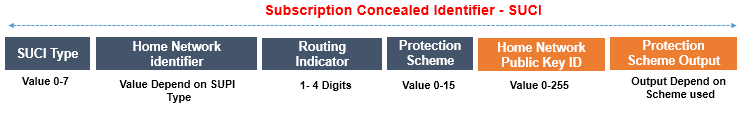
\includegraphics[width=0.8\textwidth]{images/5g-suci.png}
    \caption{Composizione del SUCI nel 5G}
\end{figure}

\section{Replicazione dell'attacco SIM-less}
Alla base degli attacchi trattati nella sezione 6.3 vi è la costruzione di un \textit{database} di \gls{imsi}. Questo \textit{database} può essere agevolmente costruito nelle generazioni precedenti al 5G 
tramite le tecniche di \gls{imsi} \textit{catching} trattate in 6.2. Nel 5G risulta molto più difficile creare un archivio di IMSI poichè questi viaggiano in forma criptata nella rete, ovvero comunicando il \gls{suci}.\\
Tuttavia, se si riuscisse a ottenere comunque un \textit{database} di \gls{imsi} rubati si potrebbe ottenere un attacco dello stesso tipo di \cite{gsm-dos-simless} e \cite{umts-dos} con prestazioni migliori 
perchè il nuovo protocollo 5G NR\cite{5g-nr} per l'\textit{air interface} è stato progettato per supportare il \textit{Massive Machine Type Communications} ovvero l'\gls{iot} massivo che richiede latenze molto basse e capacità molto alte.
Per questo, sicuramente le capacità dei canali di comunicazione durante la procedura di autenticazione avrebbero un valore di TPS molto alto, sufficiente a causare un notevole degradamento delle prestazioni.

\section{Nuove vulnerabilità}
L'implementazione del \gls{suci} e \gls{supi} ha risolto, o quantomeno reso molto più complicata la pratica dell'\gls{imsi} \textit{catching}. Allo stesso tempo però ha incrementato il dispendio di risorse durante l'autenticazione
di un dispositivo. Infatti, prima della generazione dei vettori di autenticazione vengono innestate delle procedure per decriptare il \gls{suci} con un algoritmo detto 
\gls{ecies}. 
Questa procedura aumenta inevitabilmente la creazione di possibili DOS all'autentcazione. 
In \cite{5g-lightweight} è descritto un protocollo che permetterebbe di controllare fin dal primo momento se il \gls{ms} ha un \gls{suci} valido senza incorrere nella decriptazione.